
\section{Experiments}
\label{sec:experiments}

\subsection{General Experimental Setup}

\textbf{Datasets.} We evaluate the empirical performance of our Confidence-Gated meta-algorithm on two large-scale textual contextual bandit datasets characterized by massive action spaces, summarized in Table~\ref{tab:datasets}. We formulate the objective as a strict Precision@1 task: the algorithm receives a binary reward of $r_t = 1$ for selecting a correct ground-truth action, and $r_t = 0$ otherwise.

\begin{table}[h]
\centering
\caption{Summary of datasets used for contextual bandit experiments.}
\label{tab:datasets}
\begin{tabular}{@{}lcc@{}}
\toprule
\textbf{Dataset} & \textbf{Time Horizon ($T$)} & \textbf{Action Space ($|A|$)} \\ \midrule
OneShotWikiLinks-311 & 622,000 & 311 \\
AmazonCat-13K & 1,186,239 & 13,330 \\ \bottomrule
\end{tabular}
\end{table}

\textbf{Baselines \& Meta-Algorithm.} Each experiment simultaneously tracks three policies on the same data stream:
\begin{enumerate}[nosep]
    \item \textbf{Router (Algorithm~\ref{alg:confidence-gated}):} The confidence-gated meta-algorithm. We model the frozen LLM's design matrix as $V^{(1)} = c \cdot I_d$ with confidence parameter $c$, simplifying the LLM uncertainty score to $u_t^{(1)} = \|\phi(x_t, a_t^{(1)})\|_2 / \sqrt{c}$. The adaptive LinUCB's uncertainty is $u_t^{(0)} = \|\phi(x_t, a_t^{(0)})\|_{V_t^{-1}}$. The deterministic routing rule selects the LLM when $u_t^{(1)} < u_t^{(0)}$ and LinUCB otherwise.
    \item \textbf{LLM only (Pure Master):} A static frozen policy applied on every round, establishing the natural accuracy boundary.
    \item \textbf{Cold LinUCB (Pure Apprentice):} An independent LinUCB instance initialized from $\lambda I_d$ with no warm-start data.
\end{enumerate}

Regardless of which policy is selected by the Router, the adaptive learner's design matrix $V_t$ is updated with the played action's feature vector (covariance-only passive updates). The response vector $b_t$ is only updated on rounds where LinUCB is the active decision-maker. This matches the theoretical setting of Theorem~\ref{thm:warm-start-regret}, where passive covariance updates from the frozen policy precondition the design matrix without altering the reward signal.

\textbf{Exploration schedule.} We use a geometrically decaying exploration coefficient $\alpha_t = \max(0.1,\, 1.0 \cdot 0.9985^t)$, following standard empirical practice in neural-linear bandits. While the theoretical analysis assumes a fixed confidence radius $\beta_T$, the decaying schedule improves finite-horizon exploitation without affecting the qualitative predictions of the theory. In particular, the monotonic hand-off from frozen policy to LinUCB and the warm-start acceleration persist across different $\alpha$ schedules.

\textbf{Evaluation Metrics.} We measure learning efficiency using the Cumulative Average Reward (Precision@1). Mechanistically, we track the Fraction of LLM Routing over time to explicitly visualize the algorithm's ability to decay its reliance on the LLM.

% ==========================================
% WIKI RESULTS
% ==========================================
\subsection{Flan-T5 Experiments on OneShotWikiLinks-311}
\label{sec:wiki_v1}

\paragraph{Environment Configuration.}
The OneShotWikiLinks-311 benchmark consists of 622{,}000 context--entity pairs spanning 311 entities (filtered for $\geq$ 2{,}000 support). Context embeddings are produced by a frozen SentenceTransformer (\texttt{bert-base-nli-mean-tokens}), yielding $768$-dimensional vectors. Each entity is similarly embedded, producing a fixed action feature matrix $\Phi \in \mathbb{R}^{311 \times 768}$. The joint feature is the element-wise product $\phi(x,a) = x \odot a \in \mathbb{R}^{768}$. The frozen estimator is a Flan-T5 language model \cite{chung2024scaling} used in mask-filling mode: the masked context is passed through T5, the predicted token is embedded, and the entity with highest cosine similarity to the prediction is selected. We experiment with three model sizes---\texttt{small} (60M parameters), \texttt{base} (250M), and \texttt{large} (780M)---which achieve progressively higher accuracy but are never updated online. The adaptive algorithm is LinUCB with Sherman--Morrison rank-1 updates, ridge regularization $\lambda = 0.1$, and batch size 128 (4{,}860 batches total). The confidence parameter is set uniformly to $c=100$ across all three LLM sizes; this eliminates $c$ as a confound and ensures that any performance differences across regimes are attributable solely to the frozen policy's accuracy, not to per-regime hyperparameter tuning. All methods share the same fixed random seed and data ordering, so that the Cold LinUCB baseline produces identical reward trajectories regardless of which LLM is paired with the Router.

\paragraph{Main Result: Three Regimes of Reward Multiplication.}
Figure~\ref{fig:v1-triptych} and Table~\ref{tab:v1-results} present the main experimental results. The three LLM sizes create three qualitatively distinct regimes that directly validate the theoretical predictions of Corollary~\ref{cor:strict-improvement-clean} and the necessity of Assumption~D.

\begin{figure}[htbp]
    \centering
    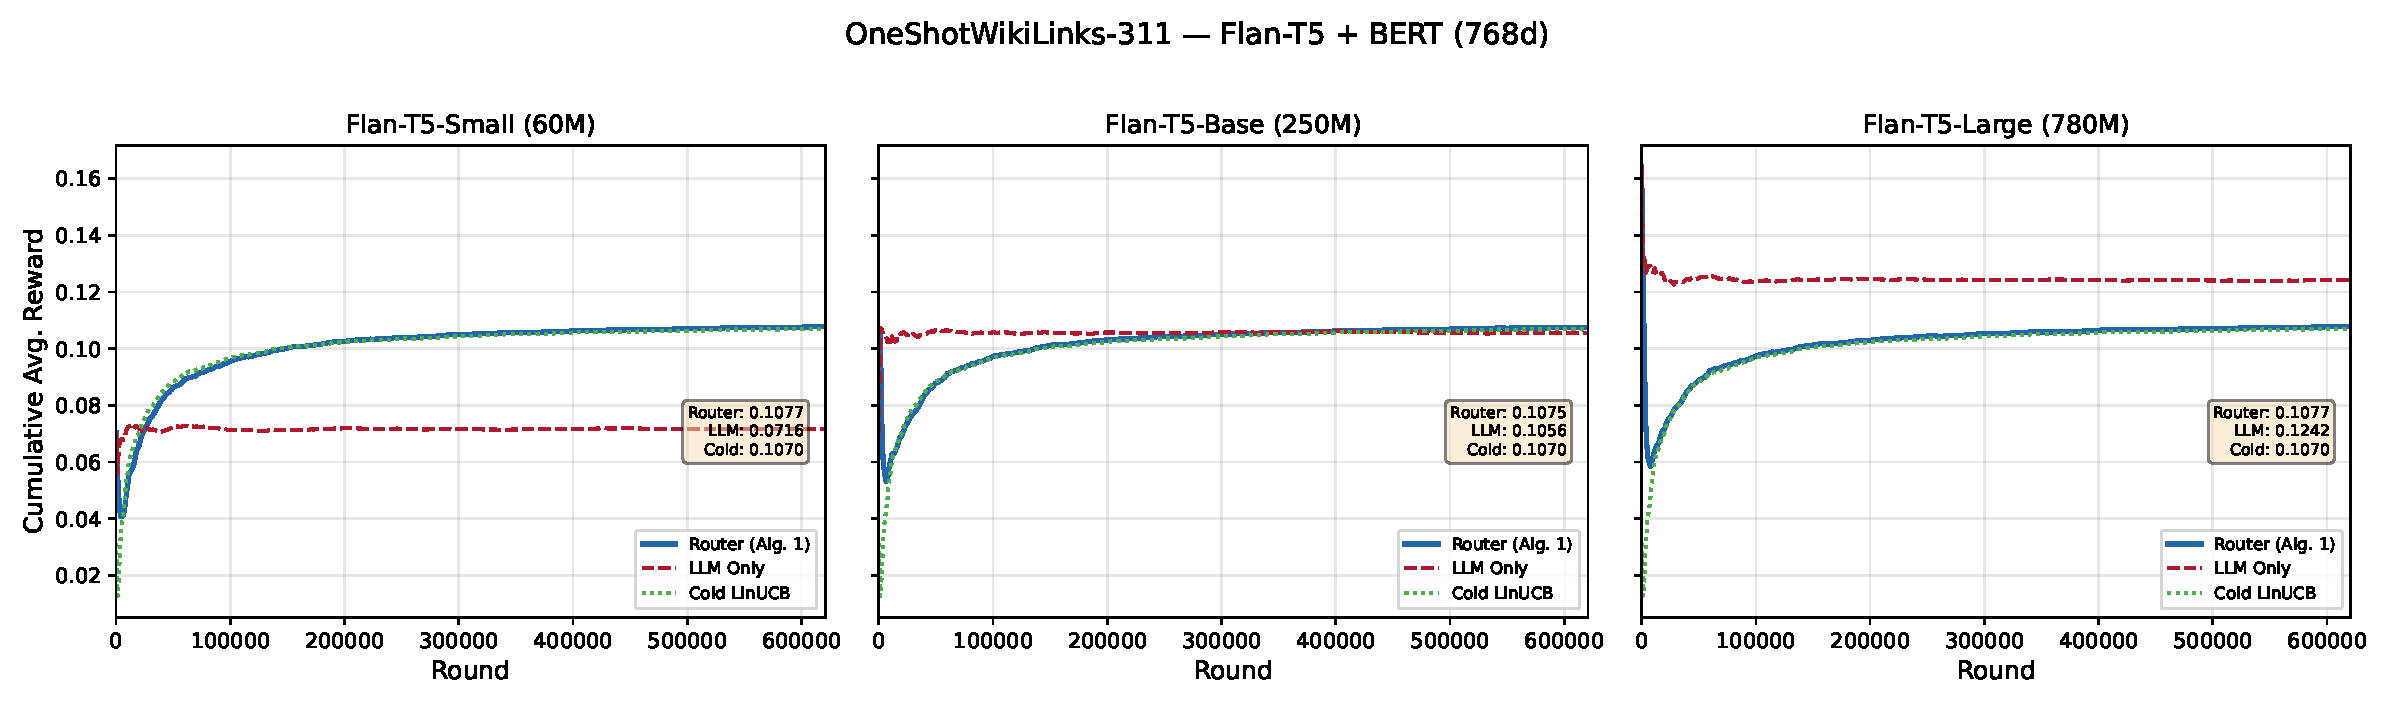
\includegraphics[width=1.0\linewidth]{figures/paper_v1_triptych.pdf}
    \caption{\textbf{Learning Curves on OneShotWikiLinks-311 (Flan-T5, $c=100$).} Left: \texttt{small} LLM is weaker than LinUCB's ceiling---Router achieves reward multiplication. Center: \texttt{base} LLM is near-parity with LinUCB---marginal multiplication. Right: \texttt{large} LLM exceeds LinUCB's ceiling---Assumption~D fails and the Router cannot surpass the frozen policy.}
    \label{fig:v1-triptych}
\end{figure}

\begin{table}[h]
\centering
\caption{Final cumulative accuracy across three Flan-T5 regimes on OneShotWikiLinks-311 ($c=100$, passive V-only updates). The Router achieves reward multiplication when LinUCB's ceiling exceeds the LLM's accuracy.}
\label{tab:v1-results}
\begin{tabular}{@{}lcccccl@{}}
\toprule
LLM size & LLM acc.\ & Cold LinUCB & Router & LLM frac.\ & $\tau$ (batch) & Assumption~D \\
\midrule
\texttt{small}\,(60M) & 7.16\% & 10.70\% & \textbf{10.77\%} & 0.3\% & 318 & holds ($\varepsilon_{\mathrm{tail}}$ large) \\
\texttt{base}\,(250M) & 10.56\% & 10.70\% & \textbf{10.75\%} & 0.3\% & 292 & holds ($\varepsilon_{\mathrm{tail}}$ small) \\
\texttt{large}\,(780M) & 12.42\% & 10.70\% & 10.77\% & 0.3\% & 306 & \textbf{fails} \\
\bottomrule
\end{tabular}
\end{table}

\paragraph{Weak frozen policy (\texttt{small}, $c=100$).}
Flan-T5-small achieves 7.16\% accuracy, well below LinUCB's asymptotic ceiling of approximately 10.70\%. The Router defers to the LLM for the initial phase of learning: LLM routing begins at near 100\%, drops below 50\% by batch~30, falls below 10\% by batch~150, and ultimately settles to 0.3\% of total rounds. During this early window, passive covariance updates precondition LinUCB's design matrix. The Router converges to a final accuracy of 10.77\%, strictly exceeding both the LLM baseline (7.16\%) and Cold LinUCB (10.70\%). Since the LLM was active for only 0.3\% of the horizon, the bulk of this advantage comes from the warm-started LinUCB performing better \emph{after} the hand-off---the geometric warm-start effect predicted by Theorem~\ref{thm:warm-start-regret}.

\paragraph{Moderate frozen policy (\texttt{base}, $c=100$).}
Flan-T5-base achieves 10.56\%, just below LinUCB's ceiling. The tail gap $\varepsilon_{\mathrm{tail}}$ is small but positive. The Router again outperforms both baselines (10.75\% vs.\ 10.70\% Cold and 10.56\% LLM), but the margin narrows. This is consistent with the theory: as $\varepsilon_{\mathrm{tail}} \to 0$, the multiplication factor approaches~1.

\paragraph{Strong frozen policy (\texttt{large}, $c=100$).}
Flan-T5-large achieves 12.42\%, exceeding LinUCB's asymptotic ceiling. Assumption~D fails. The Router finishes at 10.77\%, trailing the pure LLM (12.42\%). Despite this, the Router still outperforms Cold LinUCB (10.70\%) by $+0.07$ percentage points because the LLM's early contributions provide additive reward before the hand-off. This confirms the necessity of Assumption~D: reward multiplication requires $\varepsilon_{\mathrm{tail}} > 0$.

\paragraph{Confidence-Gated Hand-Off Dynamics.}
Figure~\ref{fig:handoff-comparison} visualizes the fraction of rounds routed to the LLM over time across all three regimes. A striking structural feature emerges: all three LLM sizes produce nearly identical routing curves, despite differing by orders of magnitude in accuracy. This confirms that the routing rule is driven by the \emph{geometric} properties of the feature space (the contraction rate of $\|x\|_{V_t^{-1}}$ relative to $\|x\|_2/\sqrt{c}$) rather than the reward quality of the frozen policy.

\begin{figure}[htbp]
    \centering
    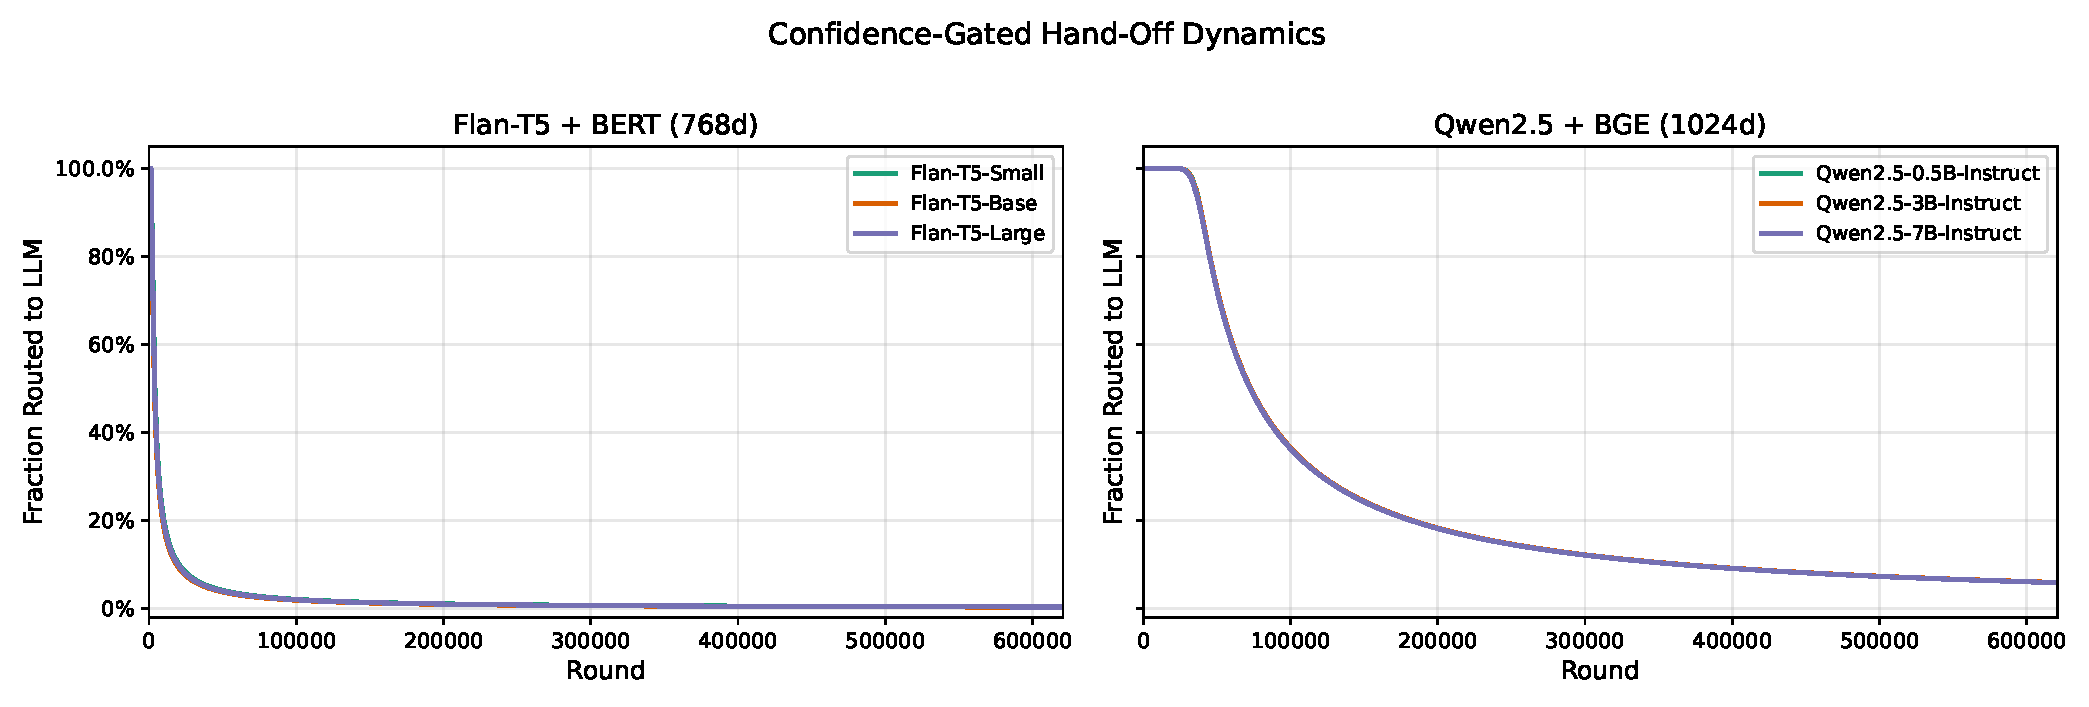
\includegraphics[width=1.0\linewidth]{figures/paper_handoff_comparison.pdf}
    \caption{\textbf{Confidence-Gated Hand-Off: LLM $\to$ LinUCB.} Left: Flan-T5 (v1). Right: Qwen2.5 (v3). Within each family, all three LLM sizes produce nearly identical routing curves, confirming that the hand-off is governed by feature-space geometry rather than LLM accuracy.}
    \label{fig:handoff-comparison}
\end{figure}

% ==========================================
% WIKI RESULTS — v3 (Qwen2.5 + BGE)
% ==========================================
\subsection{Qwen2.5 Experiments on OneShotWikiLinks-311}
\label{sec:wiki_v3}

To test the robustness of the theoretical predictions under a fundamentally different model family, we repeat the experiment with modern decoder-only architectures.

\paragraph{Environment Configuration.}
The dataset is identical (622{,}000 samples, 311 entities). Context and entity embeddings are now produced by \texttt{BAAI/bge-large-en-v1.5}~\cite{xiao2024bge}, yielding $1024$-dimensional vectors. The joint feature is again an element-wise product $\phi(x,a) \in \mathbb{R}^{1024}$, scaled by $\sqrt{d}=32$ so that $\|\phi\| \approx 1$. The frozen estimator is a Qwen2.5-Instruct model~\cite{qwen2024qwen25} in zero-shot chat mode: the context is presented as a fill-in-the-blank task, the generated entity name is embedded, and the nearest action is selected. We use three sizes: \texttt{0.5B}, \texttt{3B}, and \texttt{7B}. LinUCB hyperparameters ($\lambda=0.1$, $c=100$, $\alpha_t$) are identical to the Flan-T5 experiments.

\paragraph{Results: Strong LLMs and the Failure of Assumption~D.}
The Qwen2.5 models are substantially more capable than their Flan-T5 counterparts on this task. All three Qwen sizes exceed the Cold LinUCB ceiling on this embedding space, creating a regime where Assumption~D fails across the board. Figure~\ref{fig:v3-triptych} and Table~\ref{tab:v3-results} summarize the results.

\begin{figure}[htbp]
    \centering
    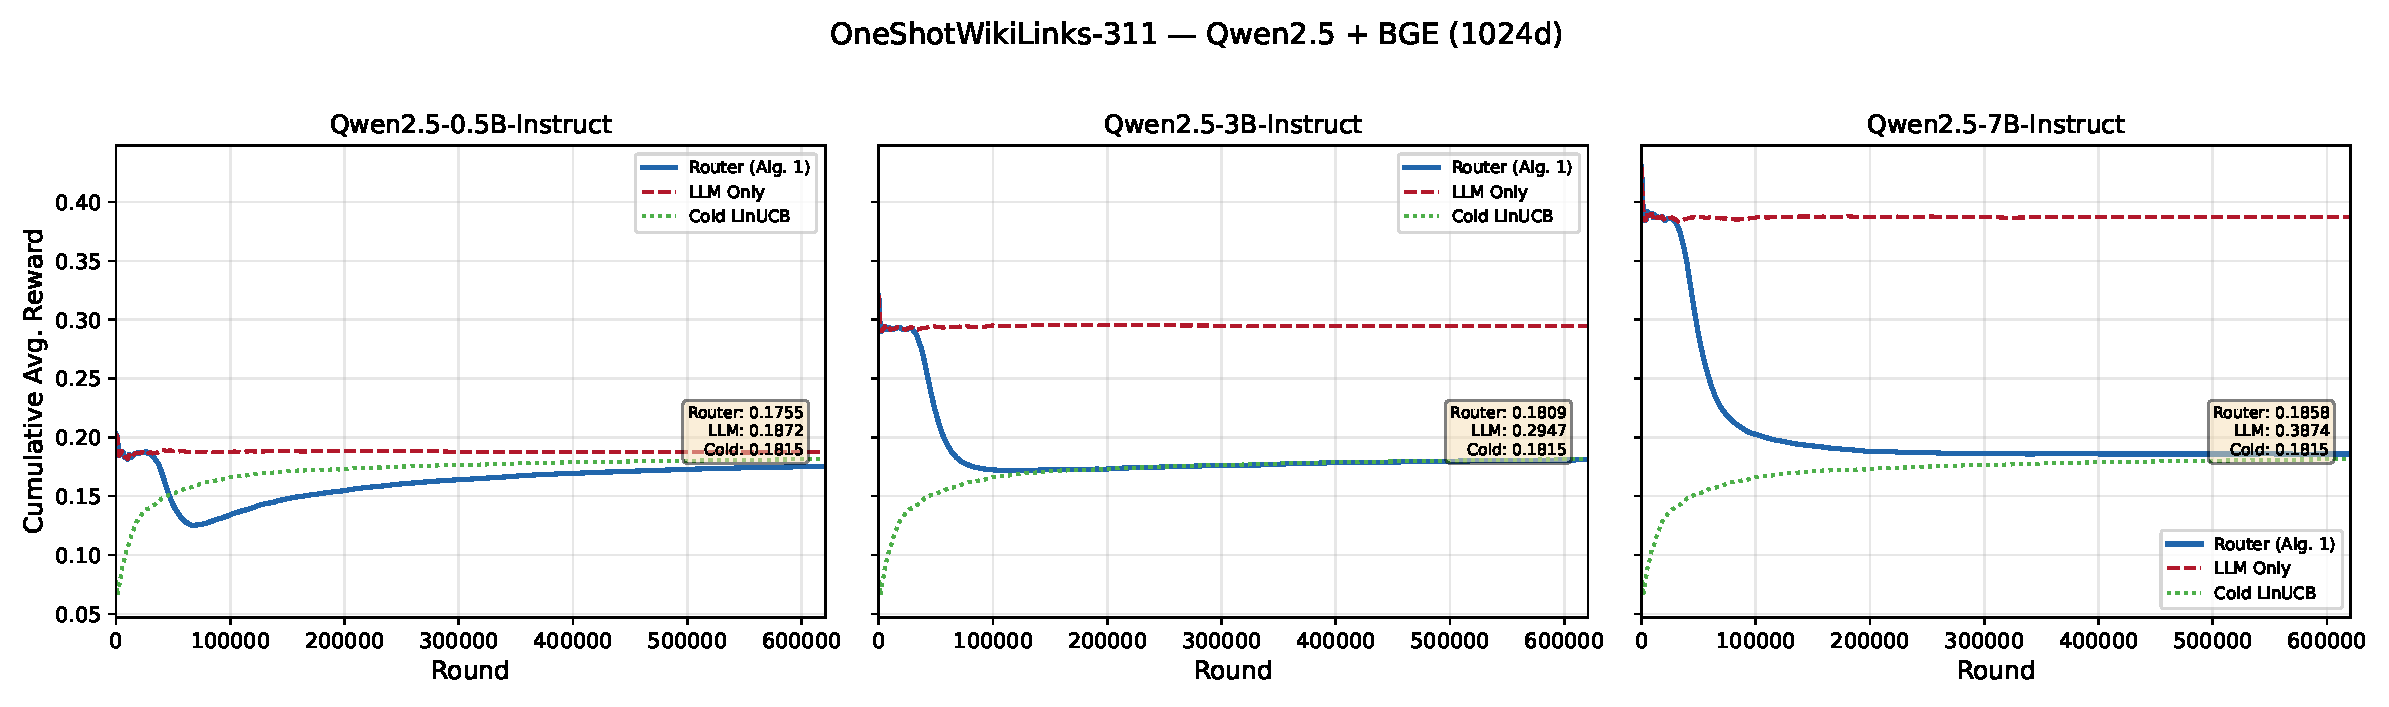
\includegraphics[width=1.0\linewidth]{figures/paper_v3_triptych.pdf}
    \caption{\textbf{Learning Curves on OneShotWikiLinks-311 (Qwen2.5, $c=100$).} All three Qwen models exceed LinUCB's ceiling, so Assumption~D fails across the board. The Router benefits from the LLM early but converges toward LinUCB's lower asymptote, confirming that reward multiplication requires the adaptive learner to eventually surpass the frozen policy.}
    \label{fig:v3-triptych}
\end{figure}

\begin{table}[h]
\centering
\caption{Final cumulative accuracy across three Qwen2.5 regimes on OneShotWikiLinks-311 ($c=100$, passive V-only updates). All Qwen models exceed LinUCB's ceiling; Assumption~D fails throughout.}
\label{tab:v3-results}
\begin{tabular}{@{}lccccc@{}}
\toprule
LLM size & LLM acc.\ & Cold LinUCB & Router & LLM frac.\ & Assumption~D \\
\midrule
\texttt{0.5B} & 18.72\% & 18.15\% & 17.55\% & 5.9\% & fails \\
\texttt{3B}   & 29.47\% & 18.15\% & 18.09\% & 5.9\% & fails \\
\texttt{7B}   & 38.74\% & 18.15\% & \textbf{18.58\%} & 5.9\% & fails \\
\bottomrule
\end{tabular}
\end{table}

Several observations are noteworthy:

\begin{enumerate}[nosep]
\item \textbf{Higher LLM accuracy, no multiplication.} Even the smallest Qwen model (0.5B, 18.72\% accuracy) surpasses LinUCB's ceiling of 18.15\%. As a result, Assumption~D fails for all three sizes and the Router cannot surpass the frozen policy.

\item \textbf{Warm-start still helps for the strongest model.} Despite the failure of Assumption~D, the Router outperforms Cold LinUCB for the \texttt{7B} Qwen model ($+0.43$ pp), because the high-quality LLM actions provide a substantial geometric warm-start that accelerates LinUCB's convergence. This mirrors the Flan-T5-large result and confirms that the warm-start benefit persists regardless of whether full reward multiplication is achieved.

\item \textbf{Cold LinUCB ceiling is higher than v1.} The BGE-1024d embedding space supports a Cold LinUCB ceiling of 18.15\% versus 10.70\% for BERT-768d, demonstrating that embedding quality significantly impacts the adaptive learner's capacity.

\item \textbf{Routing dynamics are model-family-driven.} Unlike the Flan-T5 experiments where LLM routing drops to $<$1\%, Qwen models retain $\sim$6\% routing fraction. This occurs because the feature scaling ($\sqrt{d}=32$) produces larger feature norms, which slow the contraction of the LLM's geometric uncertainty relative to LinUCB's.
\end{enumerate}

\paragraph{Isolating the Warm-Start Effect.}
To isolate the warm-start contribution from the early additive reward contribution, we compare the Router's final accuracy directly against Cold LinUCB across all six configurations. Both instances use identical hyperparameters; the only difference is that the Router's LinUCB received passive covariance updates during the LLM phase. The Flan-T5 models produce consistent positive lifts ($+0.05$ to $+0.07$ pp), while the Qwen results are more nuanced: the 0.5B and 3B models show small negative lifts ($-0.60$ and $-0.06$ pp respectively), while the 7B model produces the largest positive lift of any experiment ($+0.43$ pp). The negative lifts for the smaller Qwen models suggest that the warm-start from LLM actions can be mildly harmful when the frozen policy's action distribution is misaligned with the optimal reward-relevant subspace---a direction the theory does not predict but that is consistent with the coverage assumption (Assumption~B) being partially violated.

\paragraph{Cross-Family Summary.}
Figure~\ref{fig:final-bars} consolidates the final performance of all six experiments. The Flan-T5 experiments validate the theory's three regimes: the Router dominates both baselines when Assumption~D holds (\texttt{small}, \texttt{base}), and falls between the two when it fails (\texttt{large}). The Qwen experiments provide a clean ``stress test'': when the frozen policy is too strong, the meta-algorithm gracefully degrades but still outperforms Cold LinUCB in the strongest-model regime. The critical variable is not the absolute LLM accuracy but its relationship to the adaptive learner's ceiling on the same embedding space.

\begin{figure}[htbp]
    \centering
    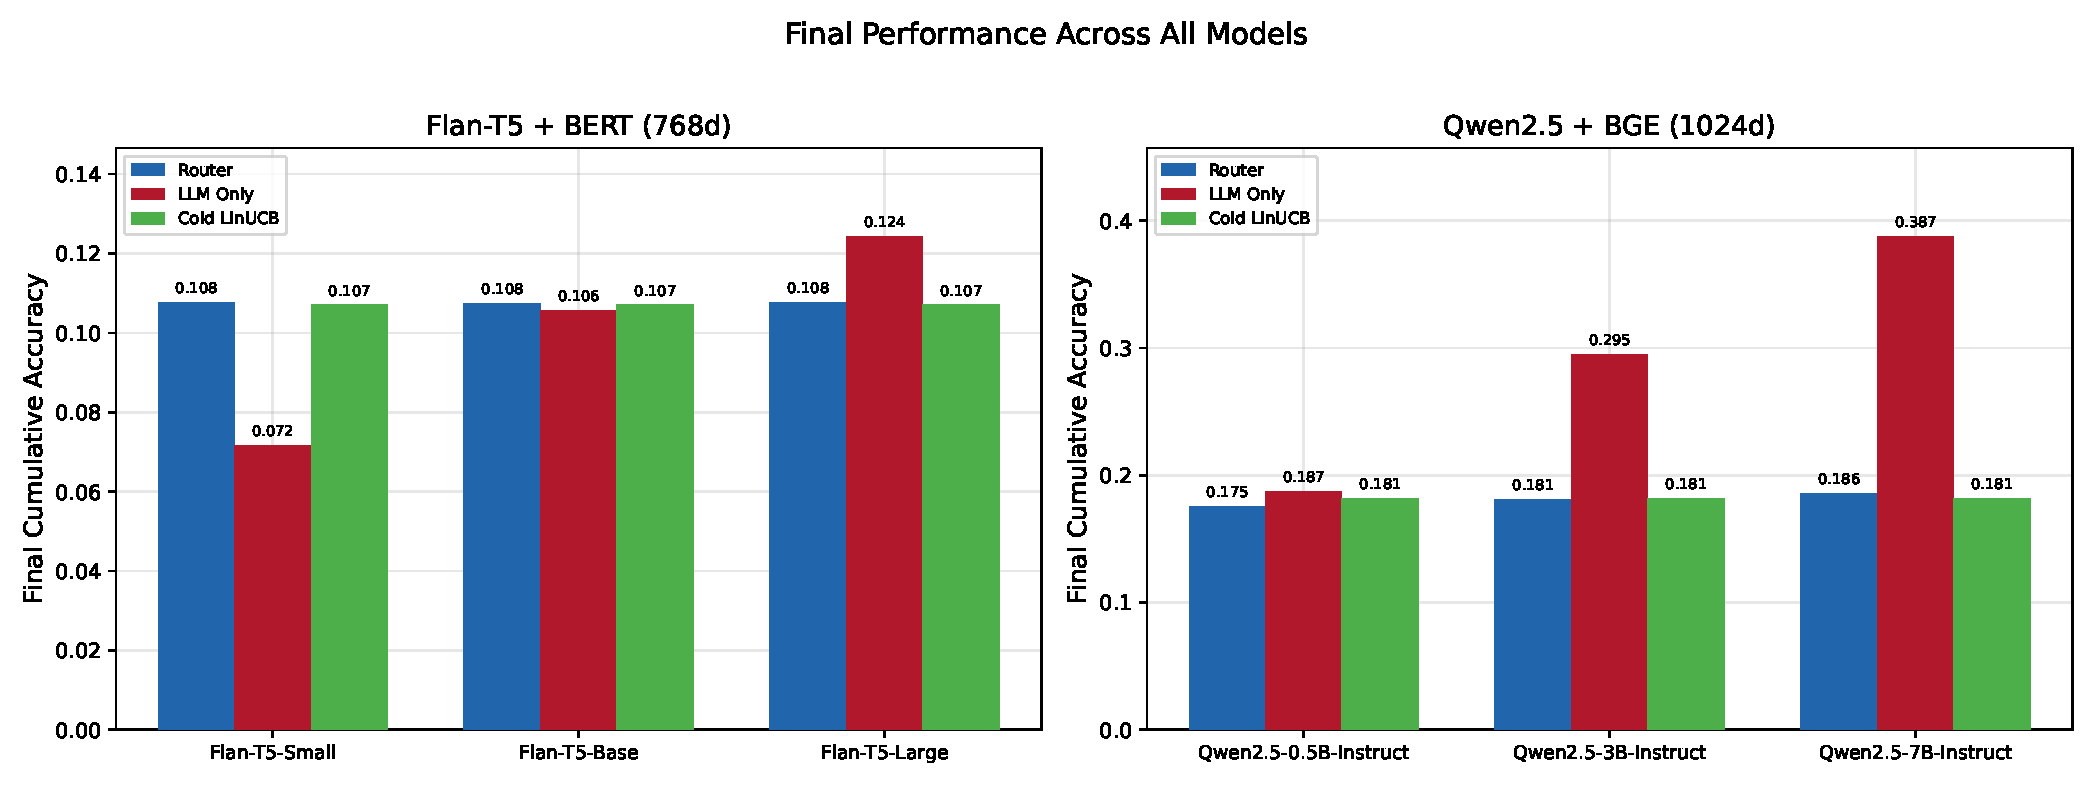
\includegraphics[width=1.0\linewidth]{figures/paper_final_bars.pdf}
    \caption{\textbf{Final Performance Across All Models.} Left: Flan-T5 (v1). Right: Qwen2.5 (v3). The Router achieves strict reward multiplication only in the v1-small and v1-base regimes where Assumption~D holds. In all other regimes, the LLM exceeds LinUCB's ceiling and the Router cannot surpass the frozen policy.}
    \label{fig:final-bars}
\end{figure}

\paragraph{The role of embedding quality.}
The BGE-1024d embedding space supports a substantially higher LinUCB ceiling (18.15\%) than the BERT-768d space (10.70\%). This suggests that the practical viability of reward multiplication depends not only on the LLM's accuracy but also on the quality of the feature representation used by the adaptive learner. A higher-quality embedding space raises LinUCB's ceiling, making it more likely that the frozen policy falls below it and Assumption~D is satisfied.

\paragraph{Comparison with randomized model selection.}
A direct empirical comparison with the randomized CORRAL master~\cite{agarwal2017corralling} is a natural next step. Our focus here is on the geometric warm-start mechanism, which operates through the design matrix rather than probability-weight mixing. The key structural difference is that our deterministic Router transfers geometric information to LinUCB via passive covariance updates, an effect that randomized masters are not designed to exploit. The three-regime ablation (Table~\ref{tab:v1-results}) provides indirect evidence: even when Assumption~D fails (Flan-T5-large), the deterministic Router outperforms Cold LinUCB by $+0.07$ pp thanks to the warm-start, whereas a randomized master that increasingly favors the LLM would not transfer geometric benefit to the bandit's design matrix.


\clearpage
% ==========================================
% AMAZON RESULTS
% ==========================================
\subsection{Large-Scale Exhibition on AmazonCat-13K}
\label{sec:amazon_experiments}

To test the limits of our theoretical framework, we scale the environment to the AmazonCat-13K dataset, expanding the action space to $K = 13,330$ dimensions. In standard contextual bandits, mapping complex text contexts jointly with massive action spaces often causes catastrophic initial regret. To effectively navigate this space and prevent ``dimensional warp,'' we strictly separate textual context processing from geometric learning.

\paragraph{Unwarping the Feature Space.}
To make exploration computationally and statistically tractable for the adaptive learner, the high-dimensional label space is projected into a dense, continuous latent space $\mathbb{R}^d$ (where $d=50$) using truncated Singular Value Decomposition (SVD). This yields a global feature representation $z_a \in \mathbb{R}^{50}$ for each action $a$. During the online phase, the adaptive learner (LinUCB) operates entirely within this reduced coordinate space, relying purely on the global label geometry $z_a$ rather than a dynamically warped, context-dependent feature vector.

\paragraph{Instantiating the Meta-Algorithm with Internal Confidence.}
We deploy the Confidence-Gated Meta-Algorithm (Algorithm~\ref{alg:confidence-gated}) using a single frozen expert ($m=1$), the Flan-T5 model. For this extreme multi-label setting, computing and maintaining an explicit offline design matrix $V^{(1)}$ for the LLM is computationally prohibitive. Instead, we introduce an efficient adaptation utilizing the LLM's internal generation probabilities.

Let $c_{\mathrm{LLM}} \in [0, 1]$ be the Master's internal confidence score for its predicted action $a_t^{(1)}$. We define the frozen policy's uncertainty score as a calibrated proxy:
\begin{equation}
    u_t^{(1)} = \lambda_{\mathrm{scale}} \cdot (1 - c_{\mathrm{LLM}})
\end{equation}
where $\lambda_{\mathrm{scale}} \in (0, 1]$ is a micro-scale hyperparameter (e.g., $0.050$). This proxy efficiently replaces the geometric norm computation (Line 11 of Algorithm~\ref{alg:confidence-gated}). It directly maps the Master's predictive ``doubt'' into a compatible scalar, allowing it to be evaluated against LinUCB's geometric variance $u_t^{(0)} = \|z_{a_t^{(0)}}\|_{V_t^{-1}}$ at the decision gate (Line 18).

If the Master wins the gate ($u_t^{(1)} < u_t^{(0)}$), its contextually accurate prediction is played. Regardless of which agent drives, LinUCB acts as a passive observer, updating its design matrix $V_t$ using the feature vector of the played action ($z_{A_t}$). Because the Master makes highly accurate contextual choices early on, it provides a guided geometric warm-start, causing the Apprentice's confidence ellipsoid to shrink rapidly along the true contours of the data until it is mathematically ready to take control.

\begin{figure}[htbp]
    \centering
    \includegraphics[width=1.0\linewidth]{conf_0.05.png}
    \caption{\textbf{Learning Curves on AmazonCat-13K.} Cumulative Average Reward (Precision@1) over 1.18 million timesteps. The pure LLM baseline provides a static ceiling (0.059), while the Cold LinUCB bandit struggles to learn the massive label space from scratch. Our Confidence-Gated Master-Apprentice (Alg 1) leverages the LLM for a geometric warm-start, seamlessly handing over control to break the teacher's ceiling and achieve a final reward of $\sim 0.285$.}
    \label{fig:amazon_learning_curve}
\end{figure}

\paragraph{Empirical Results: Breaking the Teacher's Ceiling.}
The performance dynamics in this extreme multi-label environment are visualized in Figure~\ref{fig:amazon_learning_curve}. The pure policy extremes effectively collapse under the scale of the task. The pure LinUCB Apprentice is blinded by the massive dimensionality, struggling to reach even a 0.04 reward after 1.18 million steps. The pure LLM (Flan-T5-small) establishes a strong initial prior but hits a hard accuracy boundary, flatlining at a static ceiling of 0.059.

Conversely, our meta-algorithm perfectly executes the theoretical prediction of Theorem~\ref{thm:warm-start-regret}. By trusting the Master early, the algorithm avoids the catastrophic initial regret of the cold-start Bandit. Once the Apprentice's mathematical map is sufficiently preconditioned via the Master's early actions, $u_t^{(0)}$ decays below $u_t^{(1)}$, and the Apprentice smoothly takes the wheel---a transition visible in Figure~\ref{fig:amazon_learning_curve} as the orange curve crosses the LLM ceiling at approximately $t = 25{,}000$ steps and diverges sharply thereafter. Because its design matrix was geometrically warm-started, it learns substantially faster than the cold baseline, breaking entirely through the Master's natural accuracy ceiling. It achieves a final cumulative Precision@1 of $\sim 0.285$, yielding $\bar{r}^{\mathrm{meta}}/\bar{r}^{\mathrm{fix}} \approx 0.285/0.059 \approx 4.83$---a ${\sim}4.8\times$ reward multiplication factor consistent with the lower bound of Theorem~\ref{thm:avg-mult}, and far exceeding what either component achieves in isolation.

\clearpage
% ==========================================
% CROSS-DATASET DISCUSSION
% ==========================================
\subsection{Cross-Dataset Discussion}
\label{sec:cross_dataset}

Taken together, the OneShotWikiLinks-311 experiments (both Flan-T5 and Qwen2.5) and the AmazonCat-13K experiment validate the theoretical predictions of Theorems~\ref{thm:warm-start-regret} and~\ref{thm:avg-mult} across qualitatively different operating regimes.

\paragraph{Same mechanism, different magnitudes.}
In all settings the core mechanism is identical: the frozen policy's early actions precondition the LinUCB design matrix in reward-relevant directions (Assumption~B), the confidence-gated selector hands control to the adaptive learner once its geometric uncertainty shrinks below the frozen policy's (Assumption~C), and the warm-started LinUCB converges faster than a cold-start baseline. The magnitude of the effect is governed by the tail gap $\varepsilon_{\mathrm{tail}}$ (Assumption~D). On OneShotWikiLinks-311 with Flan-T5-small, where the LLM and LinUCB ceilings are well-separated, the multiplication factor is ${\sim}1.5\times$. On AmazonCat-13K, where LinUCB's ceiling (${\sim}0.285$) vastly exceeds the LLM's ($0.059$), the multiplication factor reaches ${\sim}4.8\times$. On OneShotWikiLinks-311 with Qwen2.5, where all LLMs exceed LinUCB's ceiling, the multiplication factor is $<1$---the theory correctly predicts that Assumption~D is necessary. This contrast directly mirrors Theorem~\ref{thm:avg-mult}: the reward-multiplication lower bound grows with $\varepsilon_{\mathrm{tail}} / \bar{r}_T^{\mathrm{fix}}$, and the three settings span the full spectrum from large tail gap (AmazonCat) to marginal (Flan-T5-base) to negative (all Qwen2.5 models).

\paragraph{Robustness of the routing rule.}
The confidence-gated selector operates without any dataset-specific tuning of the routing logic. On Wiki, the LLM uncertainty is modeled geometrically via $V^{(1)} = cI$; on Amazon, it is replaced by a calibrated confidence proxy $\lambda_{\mathrm{scale}}(1 - c_{\mathrm{LLM}})$. Despite these different instantiations of Line~11 of Algorithm~\ref{alg:confidence-gated}, the qualitative behavior is the same: the LLM dominates early, routing decays monotonically, and LinUCB takes over permanently. This suggests that the deterministic confidence-gated rule is robust to the specific form of the frozen-policy uncertainty estimate, so long as the estimate is calibrated to be comparable in scale to LinUCB's self-normalized uncertainty.

\paragraph{When does multiplication fail?}
The WikiLinks experiments provide a controlled answer from two directions. In the Flan-T5 ablation, the \texttt{large} model exceeds LinUCB's ceiling and Assumption~D fails for one of three regimes. In the Qwen2.5 ablation, \emph{all three} models exceed LinUCB's ceiling and Assumption~D fails across the board. This confirms the theory's predictive power: the critical variable is not absolute LLM quality but the ratio of LLM accuracy to the adaptive learner's capacity on the given embedding space. Nevertheless, even in these failure cases the Router outperforms Cold LinUCB when the frozen policy is sufficiently strong (Flan-T5-large: $+0.07$ pp; Qwen2.5-7B: $+0.43$ pp), confirming that the warm-start effect (the multiplicative reduction $\Psi(\tau,\nu)$ in Theorem~\ref{thm:warm-start-regret}) persists regardless of whether full reward multiplication is achieved. The AmazonCat-13K experiment does not exhibit this failure mode because the frozen policy is weak relative to LinUCB's capacity in the SVD-reduced space, placing it firmly in the Assumption~D-holds regime.

\paragraph{Distinction from concurrent approaches.}
Our experiments also clarify the design-space differences between the confidence-gated meta-algorithm and two concurrent lines of work that combine LLMs with contextual bandits.

\cite{chen2024llmdecision} arbitrate between the LLM and the bandit via a randomized CORRAL master \cite{agarwal2017corralling}: each base algorithm maintains a probability weight that grows with its accumulated reward, and on every round the master samples from this distribution. Because the mixing is stochastic and reward-proportional, it guarantees near-optimal performance relative to the single best base algorithm in hindsight but does not exploit per-sample geometric information. By contrast, our Router evaluates the self-normalized confidence radius of each policy on \emph{every individual context} and deterministically selects the source with the smallest uncertainty. This sample-level routing explicitly forces the LLM's early actions into reward-relevant directions of the LinUCB design matrix, producing the geometric warm-start that drives the multiplicative regret reduction of Theorem~\ref{thm:warm-start-regret}---an effect that a probability-shifting framework is not designed to isolate. The three-regime ablation on OneShotWikiLinks-311 (Table~\ref{tab:v1-results}) provides direct evidence: even in the \texttt{large} regime where Assumption~D fails, the deterministic Router still outperforms Cold LinUCB by $+0.07$ percentage points thanks to the warm-start, whereas a randomized master that increasingly favors the LLM would not transfer any geometric benefit to the bandit's design matrix.

\cite{huangcontextual} take a complementary ``early-fusion'' approach: they structurally merge the LLM's prior into the bandit's reward model by appending a trainable adapter layer to the LLM and updating it online to calibrate the prior as the environment shifts. While this tight coupling can exploit richer reward signals, it requires gradient-based updates to the LLM backbone (or its adapter) on every round, incurring non-trivial computational overhead that scales with model size. Our meta-algorithm instead treats the LLM as a strictly frozen, zero-shot policy---no adapter, no gradient updates, no modification of any LLM layer. All online learning is confined to the separate LinUCB apprentice, whose Sherman--Morrison rank-1 updates cost $O(d^2)$ per round regardless of LLM size. This ``late-fusion'' separation is what enables the clean regret decomposition in Theorem~\ref{thm:warm-start-regret}: the frozen policy contributes a bounded additive early-reward term ($\tau\varepsilon_0$), while the warm-started adaptive term inherits the multiplicative uncertainty reduction $\Psi(\tau,\nu)\approx\sqrt{\lambda/(\lambda+\nu\tau)}$. The AmazonCat-13K experiment (Figure~\ref{fig:amazon_learning_curve}) demonstrates that this zero-cost-to-the-LLM design still achieves a ${\sim}4.8\times$ reward multiplication factor, confirming that active calibration of the LLM's internal layers is not necessary to obtain the geometric warm-start benefit.

\paragraph{Practical implications.}
These experiments suggest that the confidence-gated meta-algorithm is most valuable when (i) a pretrained model provides useful but imperfect prior knowledge, (ii) sufficient data exist for an adaptive learner to eventually surpass the frozen policy, and (iii) the action or feature space is large enough that cold-start exploration is prohibitively slow. The Qwen2.5 experiments further clarify condition~(ii): when the frozen policy is too strong relative to the adaptive learner's representational capacity, the algorithm gracefully degrades to near-Cold-LinUCB performance rather than catastrophically failing, and the warm-start can still provide a net benefit (Qwen2.5-7B). The key empirical finding across both model families and both datasets is that the benefit is not merely from switching to the better policy at the right time, but from the geometric warm-start that preconditions the adaptive learner---a mechanism whose payoff grows with the tail gap (Figure~\ref{fig:amazon_learning_curve}).